\documentclass[12pt]{article}
\usepackage[margin=0.75in]{geometry}
\usepackage{float}
\usepackage{multicol}
\usepackage{lmodern}
\usepackage{amssymb,amsmath}
\usepackage{ifxetex,ifluatex}
\usepackage{fixltx2e} % provides \textsubscript
\ifnum 0\ifxetex 1\fi\ifluatex 1\fi=0 % if pdftex
  \usepackage[T1]{fontenc}
  \usepackage[utf8]{inputenc}
\else % if luatex or xelatex
  \ifxetex
    \usepackage{mathspec}
    \usepackage{xltxtra,xunicode}
  \else
    \usepackage{fontspec}
  \fi
  \defaultfontfeatures{Mapping=tex-text,Scale=MatchLowercase}
  \newcommand{\euro}{€}
\fi
% use upquote if available, for straight quotes in verbatim environments
\IfFileExists{upquote.sty}{\usepackage{upquote}}{}
% use microtype if available
\IfFileExists{microtype.sty}{%
\usepackage{microtype}
\UseMicrotypeSet[protrusion]{basicmath} % disable protrusion for tt fonts
}{}
\usepackage{longtable,booktabs}
\usepackage{graphicx}
\makeatletter
\def\maxwidth{\ifdim\Gin@nat@width>\linewidth\linewidth\else\Gin@nat@width\fi}
\def\maxheight{\ifdim\Gin@nat@height>\textheight\textheight\else\Gin@nat@height\fi}
\makeatother
% Scale images if necessary, so that they will not overflow the page
% margins by default, and it is still possible to overwrite the defaults
% using explicit options in \includegraphics[width=3.5in][width, height, ...]{}
\setkeys{Gin}{width=\maxwidth,height=\maxheight,keepaspectratio}
\ifxetex
  \usepackage[setpagesize=false, % page size defined by xetex
              unicode=false, % unicode breaks when used with xetex
              xetex]{hyperref}
\else
  \usepackage[unicode=true]{hyperref}
\fi
\hypersetup{breaklinks=true,
            bookmarks=true,
            pdfauthor={Brandon LeBeau},
            pdftitle={PSQF 4143: Section 8},
            colorlinks=true,
            citecolor=blue,
            urlcolor=blue,
            linkcolor=magenta,
            pdfborder={0 0 0}}
\urlstyle{same}  % don't use monospace font for urls
\setlength{\parindent}{0pt}
\setlength{\parskip}{6pt plus 2pt minus 1pt}
\setlength{\emergencystretch}{3em}  % prevent overfull lines
\setcounter{secnumdepth}{0}

\title{PSQF 4143: Section 8}
\author{Brandon LeBeau}
\date{}

\begin{document}
\maketitle

\section{Statistical Inference}\label{statistical-inference}

\begin{itemize}
\itemsep1pt\parskip0pt\parsep0pt
\item
  Useful whenever our concern is with a larger group of subjects than
  just those on hand
\item
  Examples:

  \begin{itemize}
  \itemsep1pt\parskip0pt\parsep0pt
  \item
    Gallup polls
  \item
    Political polls
  \end{itemize}
\item
  Reasons for sampling

  \begin{enumerate}
  \def\labelenumi{\arabic{enumi}.}
  \itemsep1pt\parskip0pt\parsep0pt
  \item
    Not all of the population is accessible

    \begin{itemize}
    \itemsep1pt\parskip0pt\parsep0pt
    \item
      Too expensive to survey the entire population
    \item
      Physically or practically impossible to survey the entire
      population
    \end{itemize}
  \item
    The data collection procedure consumes the elements of the
    population

    \begin{itemize}
    \itemsep1pt\parskip0pt\parsep0pt
    \item
      Example: Wine Tasting
    \end{itemize}
  \end{enumerate}
\end{itemize}

\section{Statistical Inference 2}\label{statistical-inference-2}

\begin{itemize}
\itemsep1pt\parskip0pt\parsep0pt
\item
  The basic aim of statistical inference is to make a conclusion about a
  \textbf{population parameter} based on a \textbf{sample statistic}
  obtained from a sample of the population.
\end{itemize}

\begin{longtable}[c]{@{}lr@{}}
\toprule
Characteristic & Parameter\tabularnewline
\midrule
\endhead
Mean & \(\mu\)\tabularnewline
Standard Dev. & \(\sigma\)\tabularnewline
Correlation & \(\rho\)\tabularnewline
Median & \(\epsilon\)\tabularnewline
Proportion & \(\pi\)\tabularnewline
\bottomrule
\end{longtable}

\section{Example}\label{example}

\begin{figure}[H]
\centering
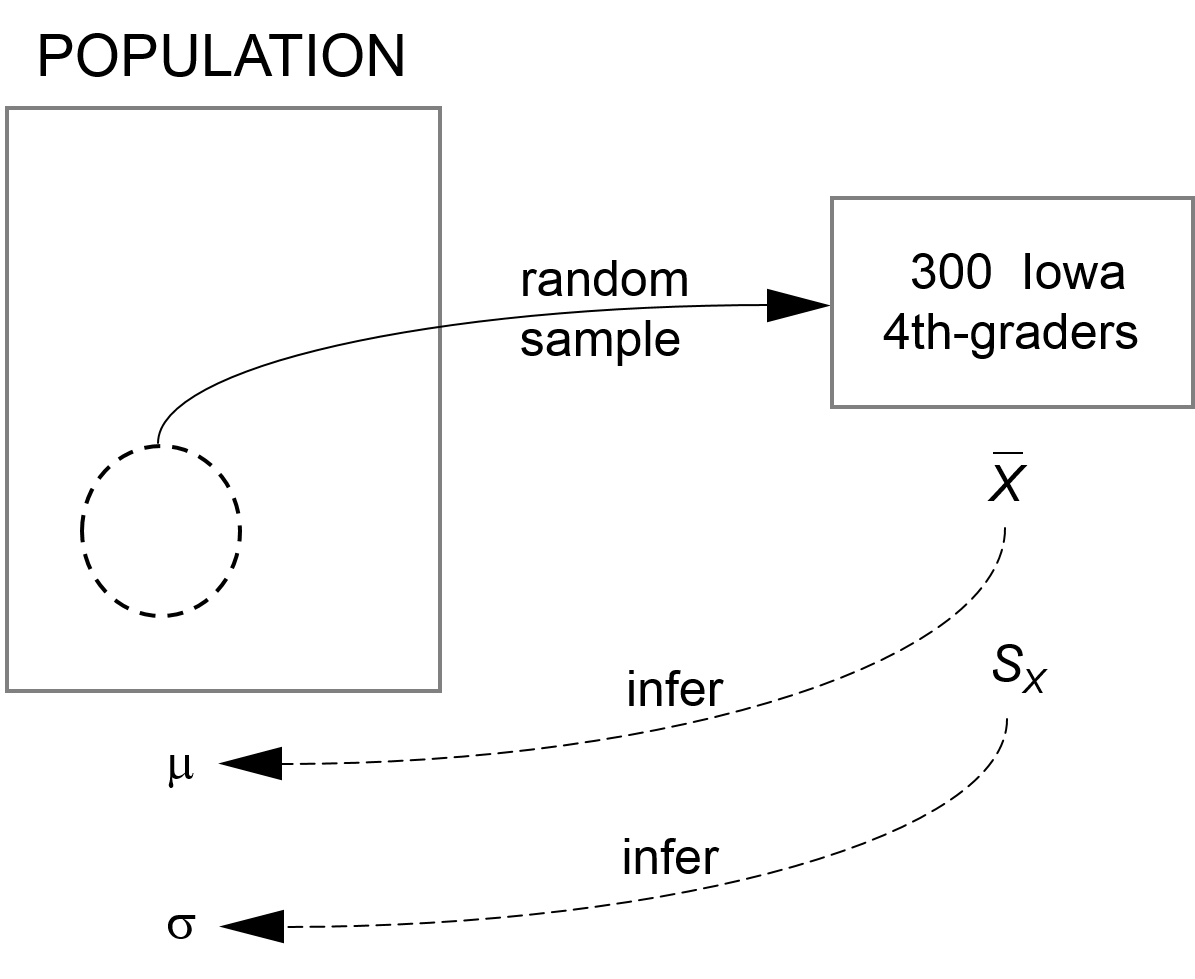
\includegraphics[width=3.5in]{itbs_infer.png}
\caption{}
\end{figure}

\section{Population Terminology}\label{population-terminology}

\begin{itemize}
\itemsep1pt\parskip0pt\parsep0pt
\item
  Experimentally Accessible Population (EAP)

  \begin{itemize}
  \itemsep1pt\parskip0pt\parsep0pt
  \item
    The population from which we sample
  \item
    The EAP is what is available to the researcher when she does her
    study
  \end{itemize}
\item
  Target Population (TP)

  \begin{itemize}
  \itemsep1pt\parskip0pt\parsep0pt
  \item
    The population to which we generalize
  \end{itemize}
\end{itemize}

\section{Population Terminology
Example}\label{population-terminology-example}

\begin{figure}[H]
\centering
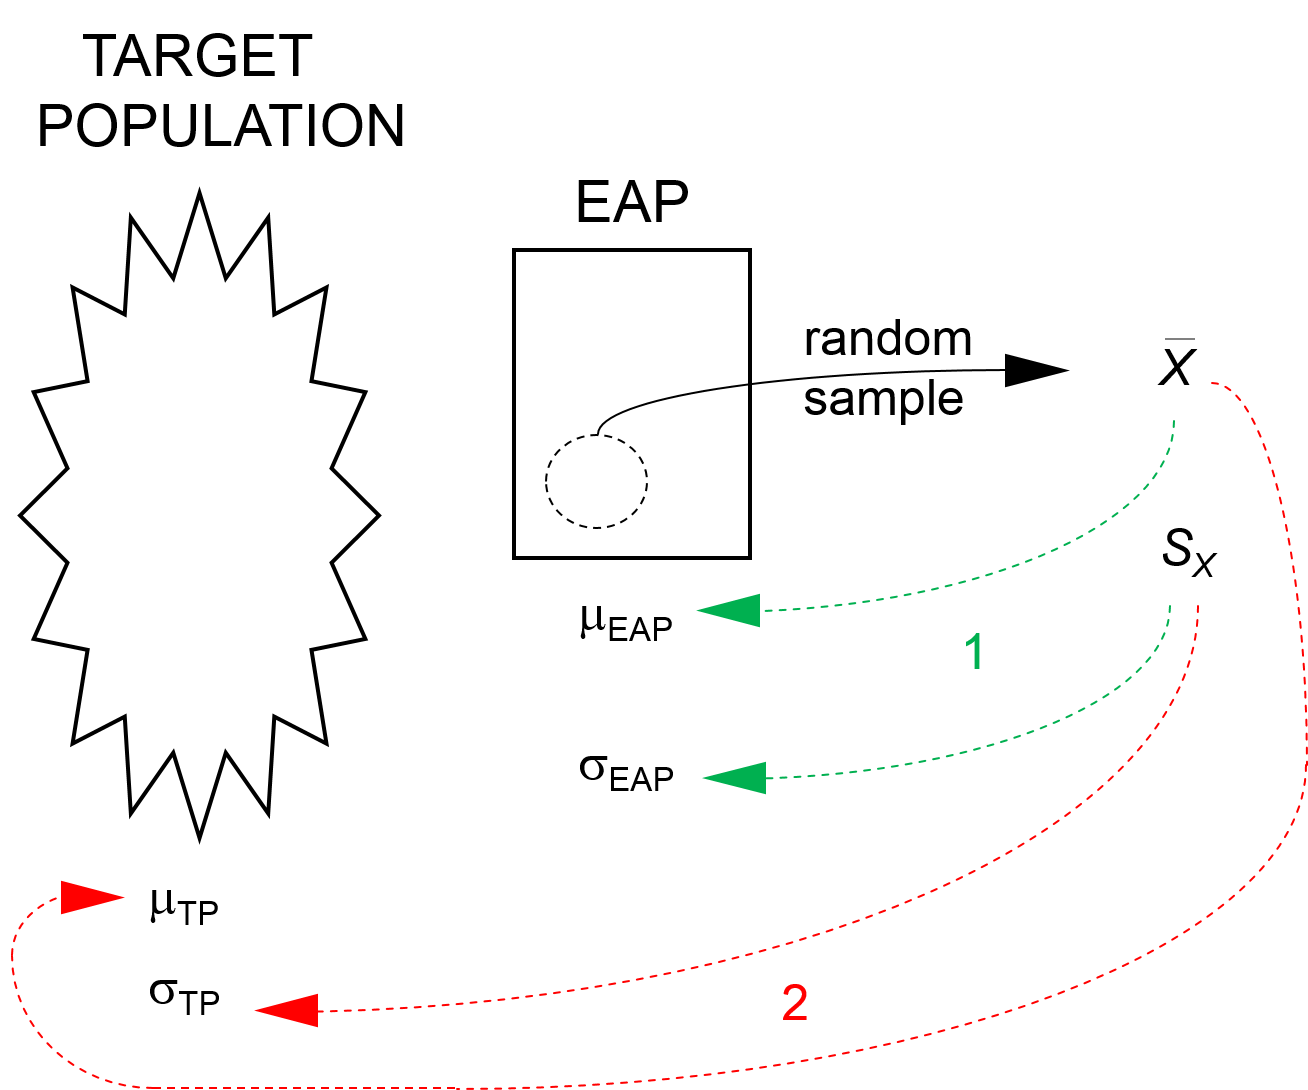
\includegraphics[width=3.5in]{infer_population.png}
\caption{}
\end{figure}

\section{Population Example 1}\label{population-example-1}

\begin{itemize}
\itemsep1pt\parskip0pt\parsep0pt
\item
  Effects of Guidance on the Results of Standardized Tests.

  \begin{itemize}
  \item
    Purpose: \textgreater{} ``to ascertain whether a group of students
    could be effectively motivated, through individual and group
    guidance activities, to achieve significantly higher results on the
    ITED than another group of students who were not afforded the same
    guidance services.''
  \item
    Subjects: \textgreater{} ``270 ninth grade students from a
    midwestern community of mixed social and ethnic background. One-half
    the students were randomly assigned to an experimental group and
    one-half to a control group''
  \item
    Conclusions: \textgreater{} ``the results of the standardized
    achievement testing were related to the motivational and teaching
    activities that were carried out prior to the testing''
    \textgreater{} ``improved test results are obtainable when students
    become personally involved in, motivated by, and interested in the
    testing program'' \textgreater{} ``All schools are interested in
    improving their . . . standardized test {[}scores{]}, but more
    important, they must be interested in the individual student and his
    development''
  \end{itemize}
\end{itemize}

\section{Population Example 2}\label{population-example-2}

\begin{itemize}
\itemsep1pt\parskip0pt\parsep0pt
\item
  The determination of Social Ranks and Roles

  \begin{itemize}
  \item
    Purpose: \textgreater{} ``Are there individual differences in the
    quality of maternal care given kids and, if there are, do these lead
    to differences in social roles?''
  \item
    Variables:

    \begin{itemize}
    \itemsep1pt\parskip0pt\parsep0pt
    \item
      speed of birth
    \item
      immediacy (latency) of maternal responses
    \item
      intensity of maternal responsiveness
    \item
      vigor of kid
    \item
      nursing latency, frequency, and duration
    \item
      weight and sex of kid
    \item
      relative dominance during play
    \item
      priority of access to mother
    \item
      spatial relations vis-a-vis other kids
    \end{itemize}
  \item
    Subjects: \textgreater{} ``a small group of inbred Toggenburg
    goats''
  \item
    Conclusions: \textgreater{} ``For goats, and other social species,
    it makes sense to diversify these capabilities as much as possible
    -- the reverse of the all-apples-in-one-basket strategy''
  \end{itemize}
\end{itemize}

\section{Population Examples Summary}\label{population-examples-summary}

\begin{itemize}
\itemsep1pt\parskip0pt\parsep0pt
\item
  In the strictest sense, the results of research studies are limited to
  generalizations directly to the EAP.
\item
  Any generalizations to the TP require logical considerations of the
  similarities and differences between the EAP and TP and how these
  difference may affect the results.

  \begin{itemize}
  \itemsep1pt\parskip0pt\parsep0pt
  \item
    This is one place where the art of science enters.
  \end{itemize}
\end{itemize}

\section{Situations where EAP and TP may
differ}\label{situations-where-eap-and-tp-may-differ}

\begin{enumerate}
\def\labelenumi{\arabic{enumi}.}
\itemsep1pt\parskip0pt\parsep0pt
\item
  Learning Experiments (cognitive function)

  \begin{itemize}
  \itemsep1pt\parskip0pt\parsep0pt
  \item
    Example: when subjects are undergraduate university students
  \end{itemize}
\item
  Methods Studies in Education

  \begin{itemize}
  \itemsep1pt\parskip0pt\parsep0pt
  \item
    Example: Method to teach fifth-graders to spell

    \begin{itemize}
    \itemsep1pt\parskip0pt\parsep0pt
    \item
      Commonly uses intact classrooms
    \end{itemize}
  \item
    Can also happen in medical research
  \end{itemize}
\item
  Polls

  \begin{itemize}
  \itemsep1pt\parskip0pt\parsep0pt
  \item
    Time factor
  \end{itemize}
\item
  Medical Studies with Animals

  \begin{itemize}
  \itemsep1pt\parskip0pt\parsep0pt
  \item
    Example: Saccharine causes cancer in rats, therefore it is banned
    from human consumption.
  \end{itemize}
\end{enumerate}

\section{Newspaper Example}\label{newspaper-example}

\begin{figure}[H]
\centering
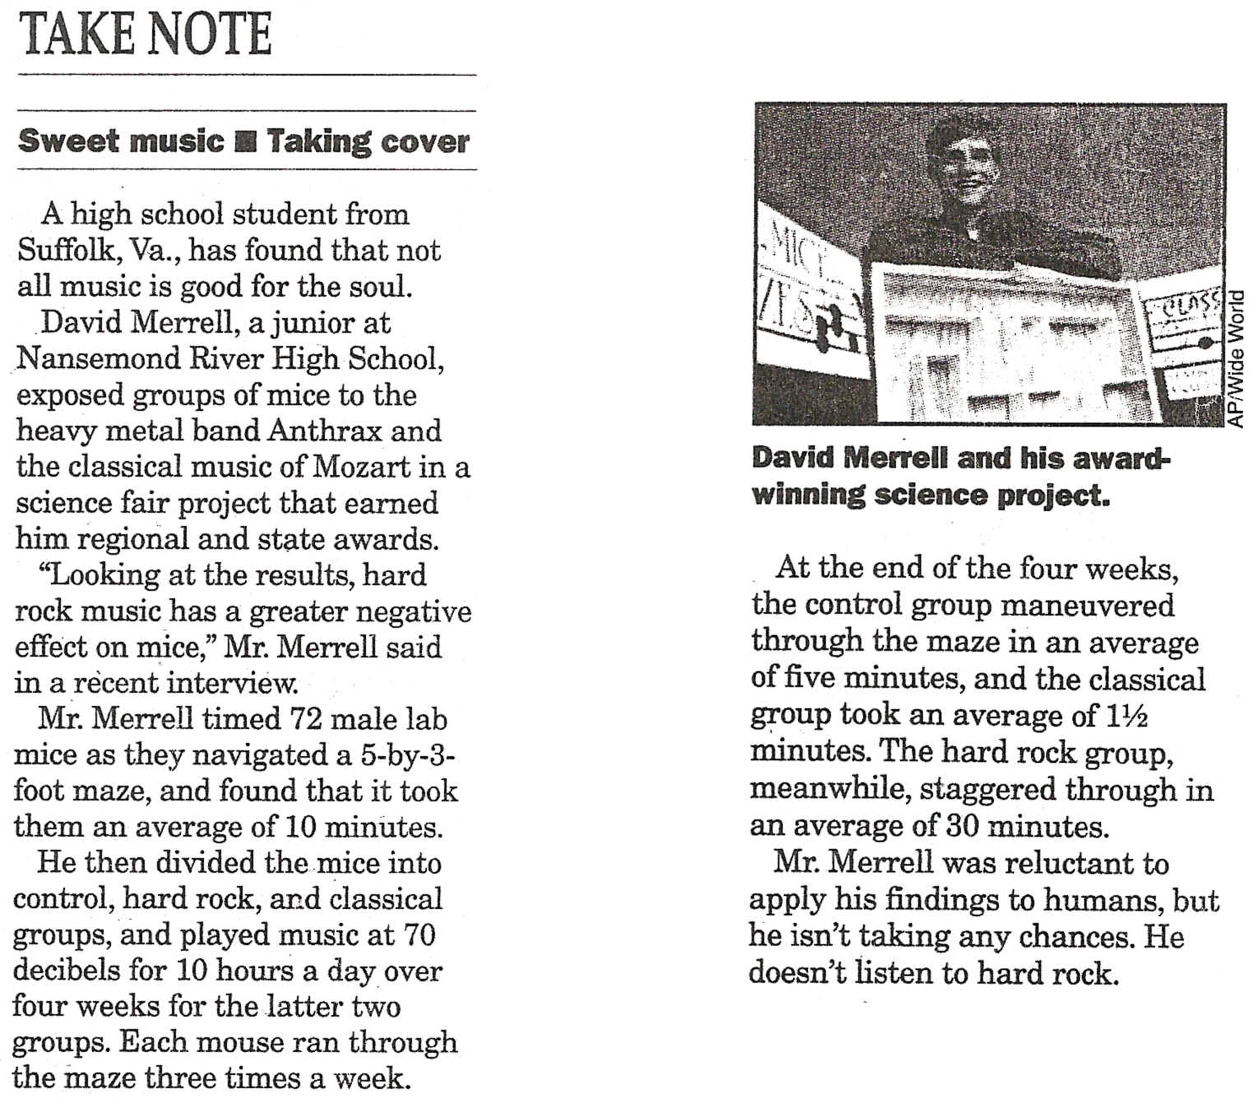
\includegraphics[width=3.5in]{science_project.png}
\caption{}
\end{figure}

\section{Random Sampling}\label{random-sampling}

\begin{itemize}
\itemsep1pt\parskip0pt\parsep0pt
\item
  A \textbf{random sample} of a given population is a sample that is
  drawn so that each possible sample of that size has an equal
  probability of being selected from the population.

  \begin{itemize}
  \itemsep1pt\parskip0pt\parsep0pt
  \item
    Note: It is the method of selection, not the particular sample
    outcome that defines a random sample.
  \end{itemize}
\end{itemize}

\section{Sampling Error}\label{sampling-error}

\begin{itemize}
\itemsep1pt\parskip0pt\parsep0pt
\item
  \textbf{Sampling Error} is the difference between the value of the
  population parameter (\(\theta\)) and that of the sample statistic
  (\(T\))

  \begin{itemize}
  \itemsep1pt\parskip0pt\parsep0pt
  \item
    \(E = T - \theta\)

    \begin{itemize}
    \itemsep1pt\parskip0pt\parsep0pt
    \item
      \(E\) is the sampling error
    \item
      \(T\) is the value of the sample statistic
    \item
      \(\theta\) is the value of the population parameter
    \end{itemize}
  \end{itemize}
\item
  The key to any situation in statistical inference is to know what
  sample values occur in repeated sampling, and with what probability.
\item
  In other words, we need to know the sampling distribution of the
  statistic.
\item
  We must be able to describe the sampling distribution of the statistic
  completely if we are to say what would happen when samples are drawn.
\end{itemize}

\section{Bias}\label{bias}

\begin{itemize}
\itemsep1pt\parskip0pt\parsep0pt
\item
  If a sample is not done randomly, then there is a biased sample.
\item
  It follows, if we have a biased sample, the sample statistic would not
  correspond to the population parameter and the sample statistic would
  be biased.
\item
  This results in \textbf{systematic error} in addition to
  random/sampling error.
\item
  Two major ways to have bias:

  \begin{enumerate}
  \def\labelenumi{\arabic{enumi}.}
  \itemsep1pt\parskip0pt\parsep0pt
  \item
    Sample selection - troublesome, no way to adjust
  \item
    Characteristic of the statistic - this we can adjust for if known.
  \end{enumerate}
\end{itemize}

\section{Sampling Distribution for the
Mean}\label{sampling-distribution-for-the-mean}

\begin{figure}[H]
\centering
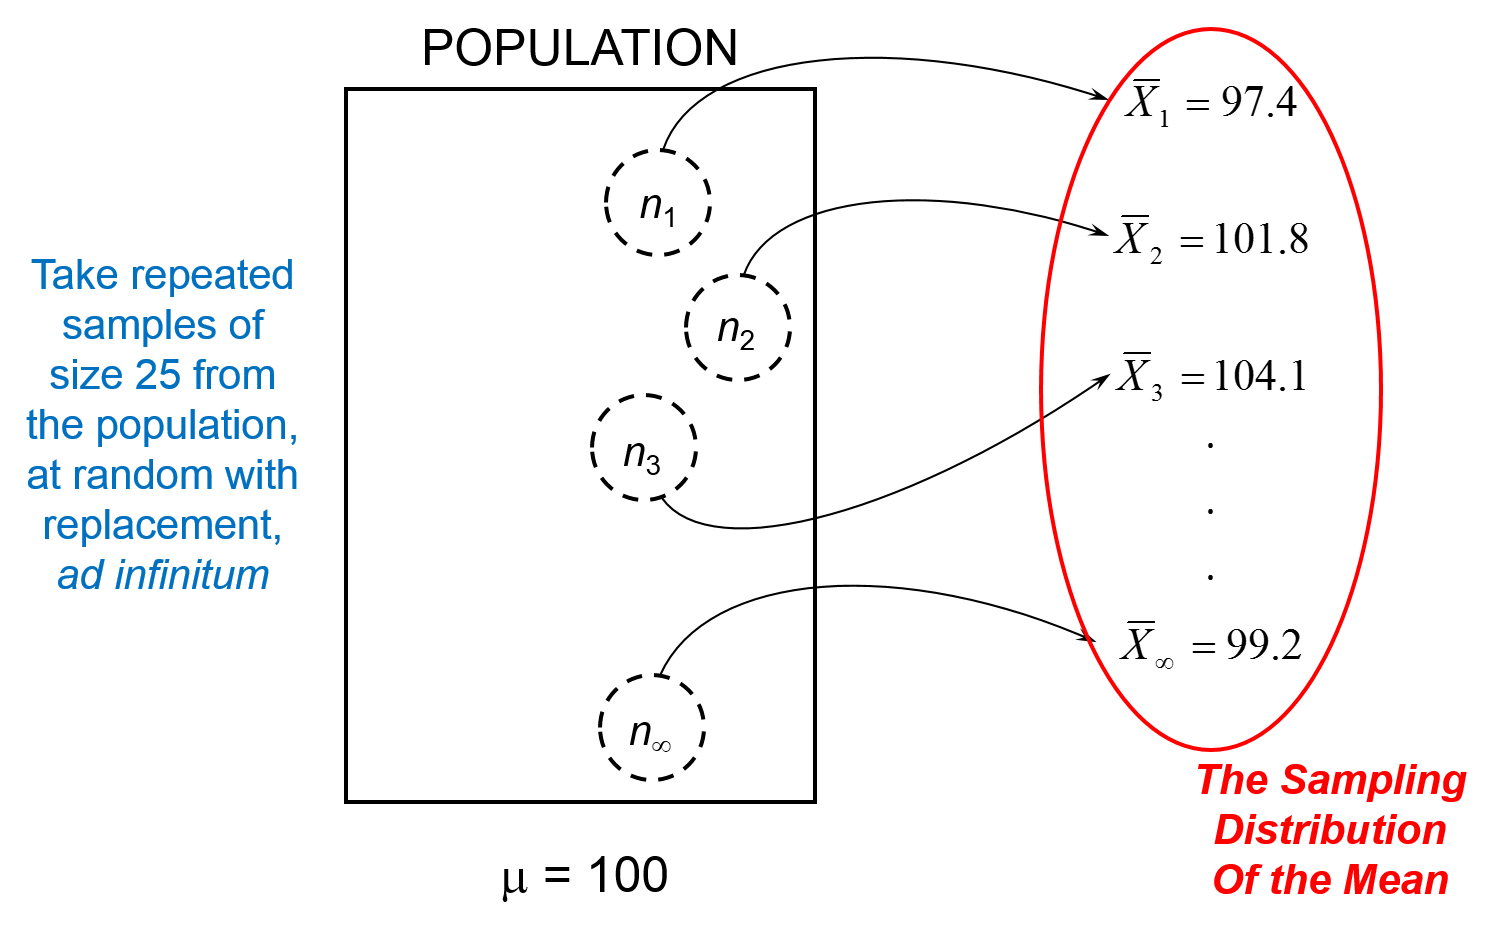
\includegraphics[width=3.5in]{sample_dist.png}
\caption{}
\end{figure}

\section{Sampling Distribution
Example}\label{sampling-distribution-example}

\begin{itemize}
\itemsep1pt\parskip0pt\parsep0pt
\item
  Suppose our population consists of 4 values: 2, 4, 6, 8
\item
  We wish to draw random samples of size 2 from this population with
  replacement.
\end{itemize}
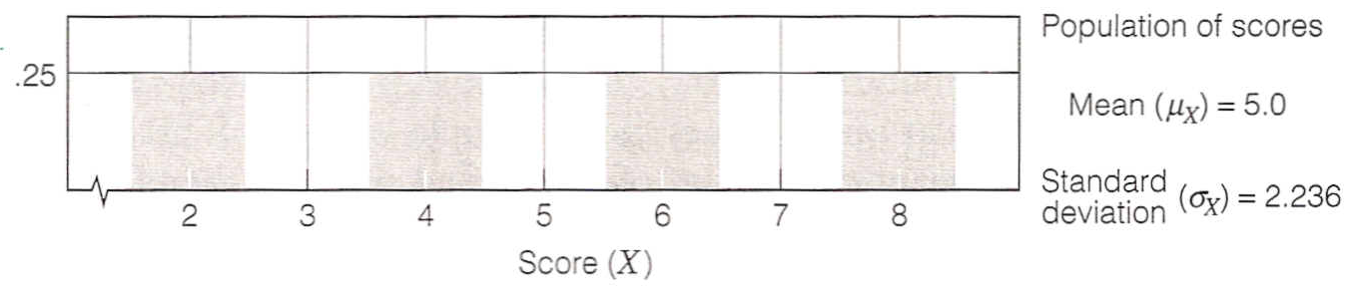
\includegraphics[width=3.5in]{sample_dist_population.png}

\section{Possible Samples}\label{possible-samples}

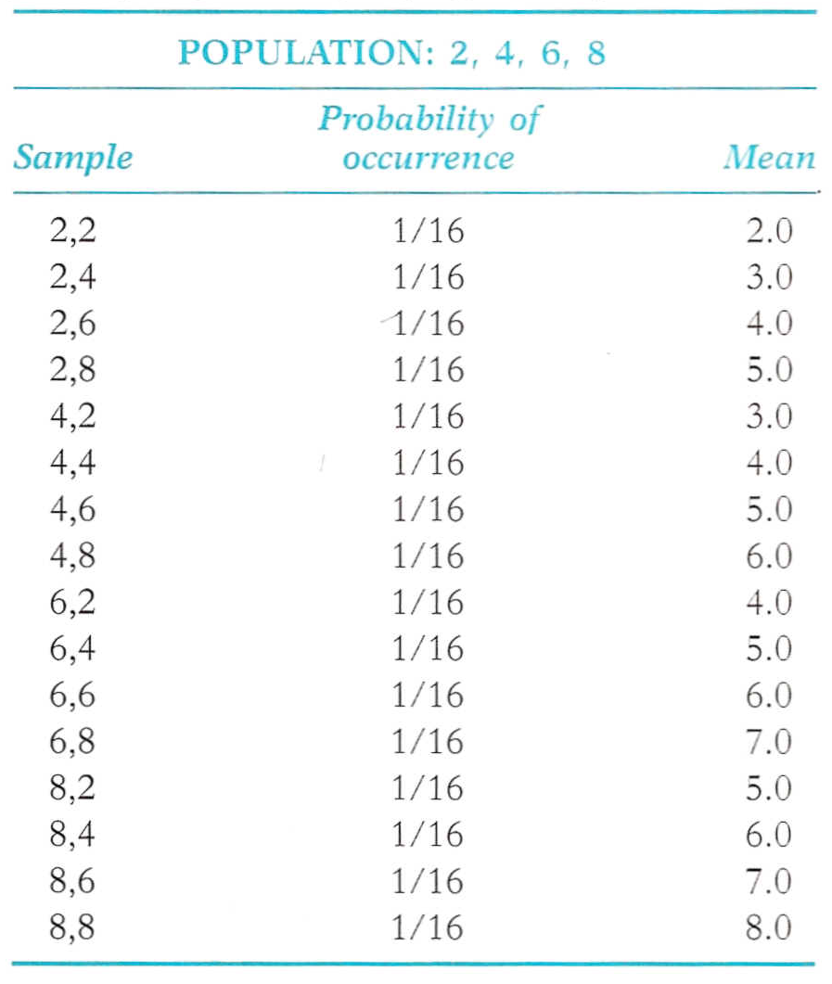
\includegraphics[width=3.5in]{sample_dist_outcomes.png}
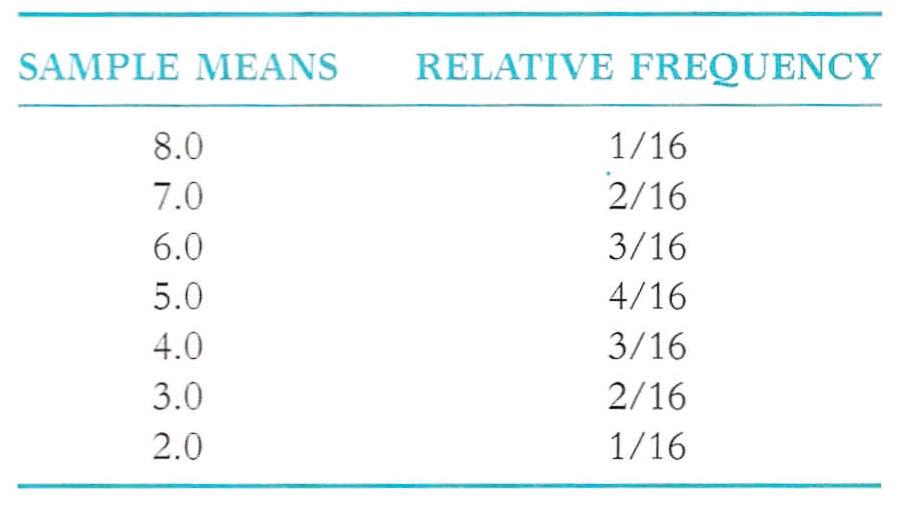
\includegraphics[width=3.5in]{sample_dist_meanout.png}

\section{Sampling Distribution of the
Mean}\label{sampling-distribution-of-the-mean}

\begin{itemize}
\itemsep1pt\parskip0pt\parsep0pt
\item
  For samples of size 2, drawn repeatedly with replacement from the
  population 2, 4, 6, 8. 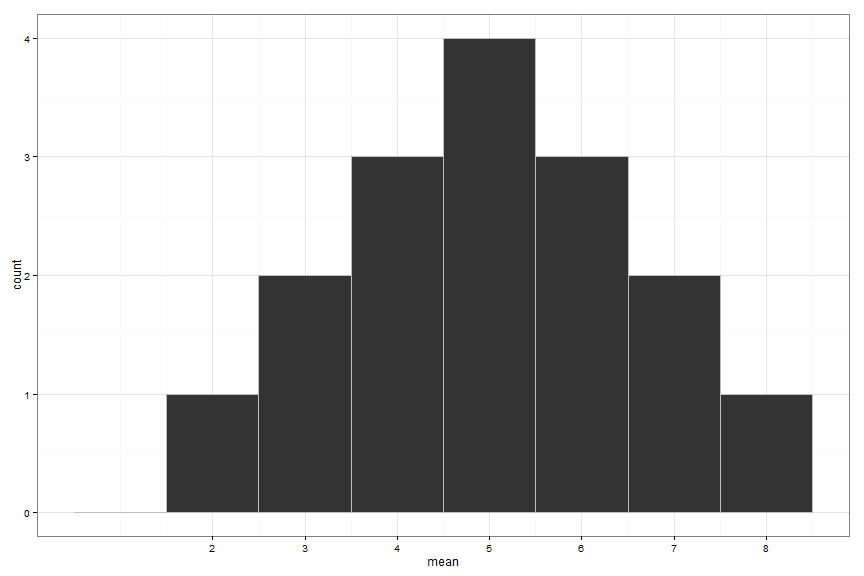
\includegraphics[width=3.5in]{figure/sampdist-1.png}
  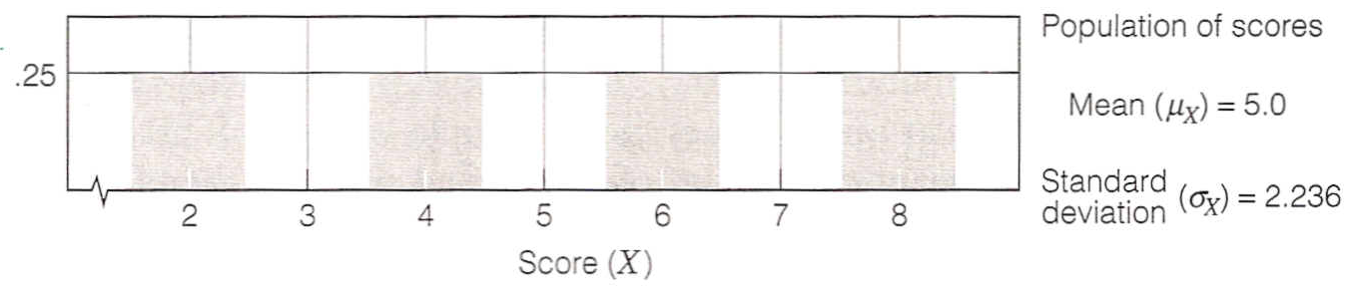
\includegraphics[width=3.5in]{sample_dist_population.png}
\end{itemize}

\section{Sampling Distribution
Process}\label{sampling-distribution-process}

\begin{figure}[H]
\centering
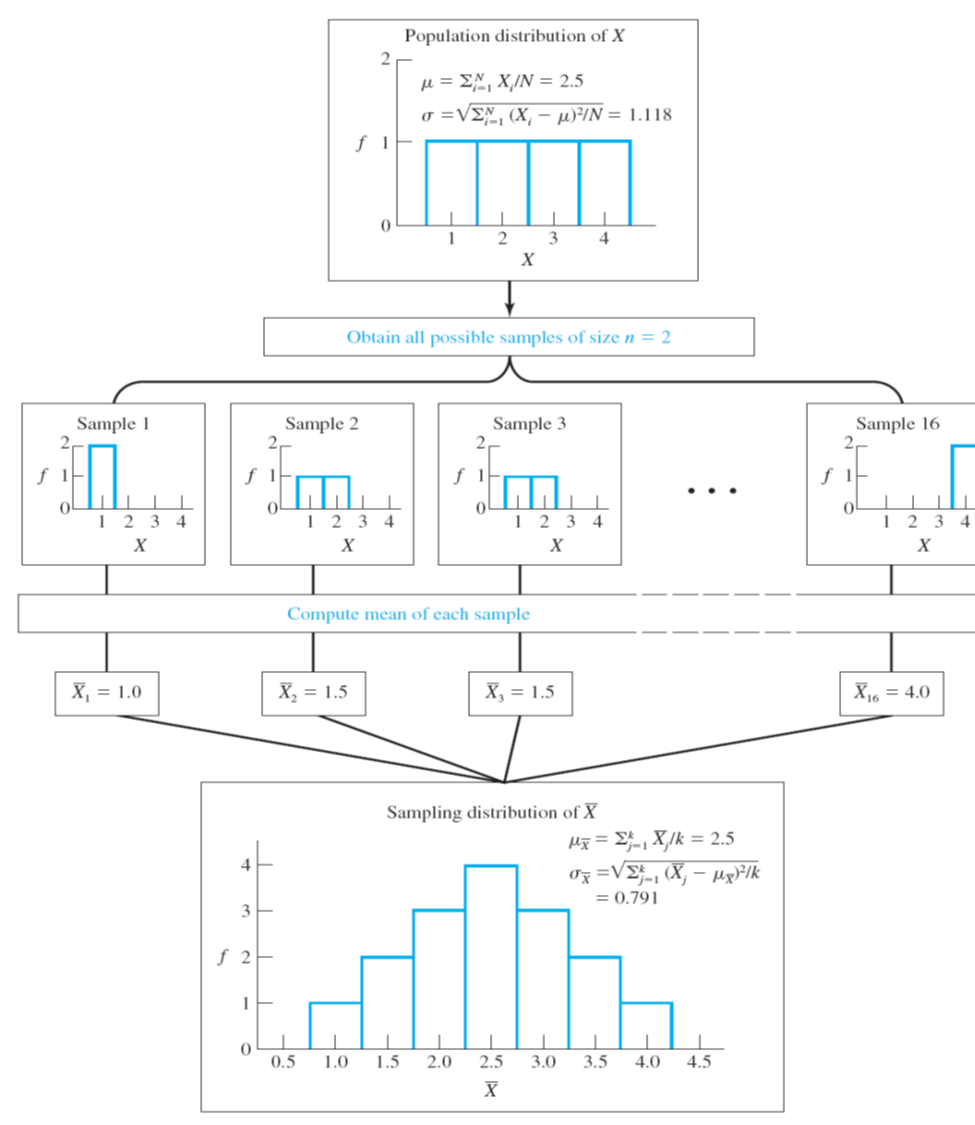
\includegraphics[width=3.5in]{sample_dist_process.png}
\caption{}
\end{figure}

\section{Sampling Distribution of the
Mean}\label{sampling-distribution-of-the-mean-1}

\begin{itemize}
\itemsep1pt\parskip0pt\parsep0pt
\item
  The mean of any random sampling distribution of \(\bar{X}\), called
  the \textbf{expected value of the sample mean}, is the same as the
  mean of the population of scores. \[\mu_{\bar{X}} = \mu_{X}\]
\item
  This is true regardless of the sample size (\(n\)), standard deviation
  (\(\sigma_{X}\)), and the shape of the population distribution.
\item
  Assumes sampling with replacement, or \(n < 5\%\) of \(N\)
\end{itemize}

\section{Sampling Distribution of the Mean
2}\label{sampling-distribution-of-the-mean-2}

\begin{itemize}
\itemsep1pt\parskip0pt\parsep0pt
\item
  The standard deviation of the sampling distribution of \(\bar{X}\),
  called the \textbf{standard error of the mean}, depends on the
  standard deviation of the population, \(\sigma_{X}\) and the sample
  size, \(n\). \[ \sigma_{\bar{X}} = \frac{\sigma_{X}}{\sqrt{n}} \]
\item
  The standard error of the mean is based on samples of a specified
  size.
\item
  Assumes sampling with replacement, or \(n < 5\%\) of \(N\)
\end{itemize}

\section{Sampling Distribution
Graphic}\label{sampling-distribution-graphic}

\begin{figure}[H]
\centering
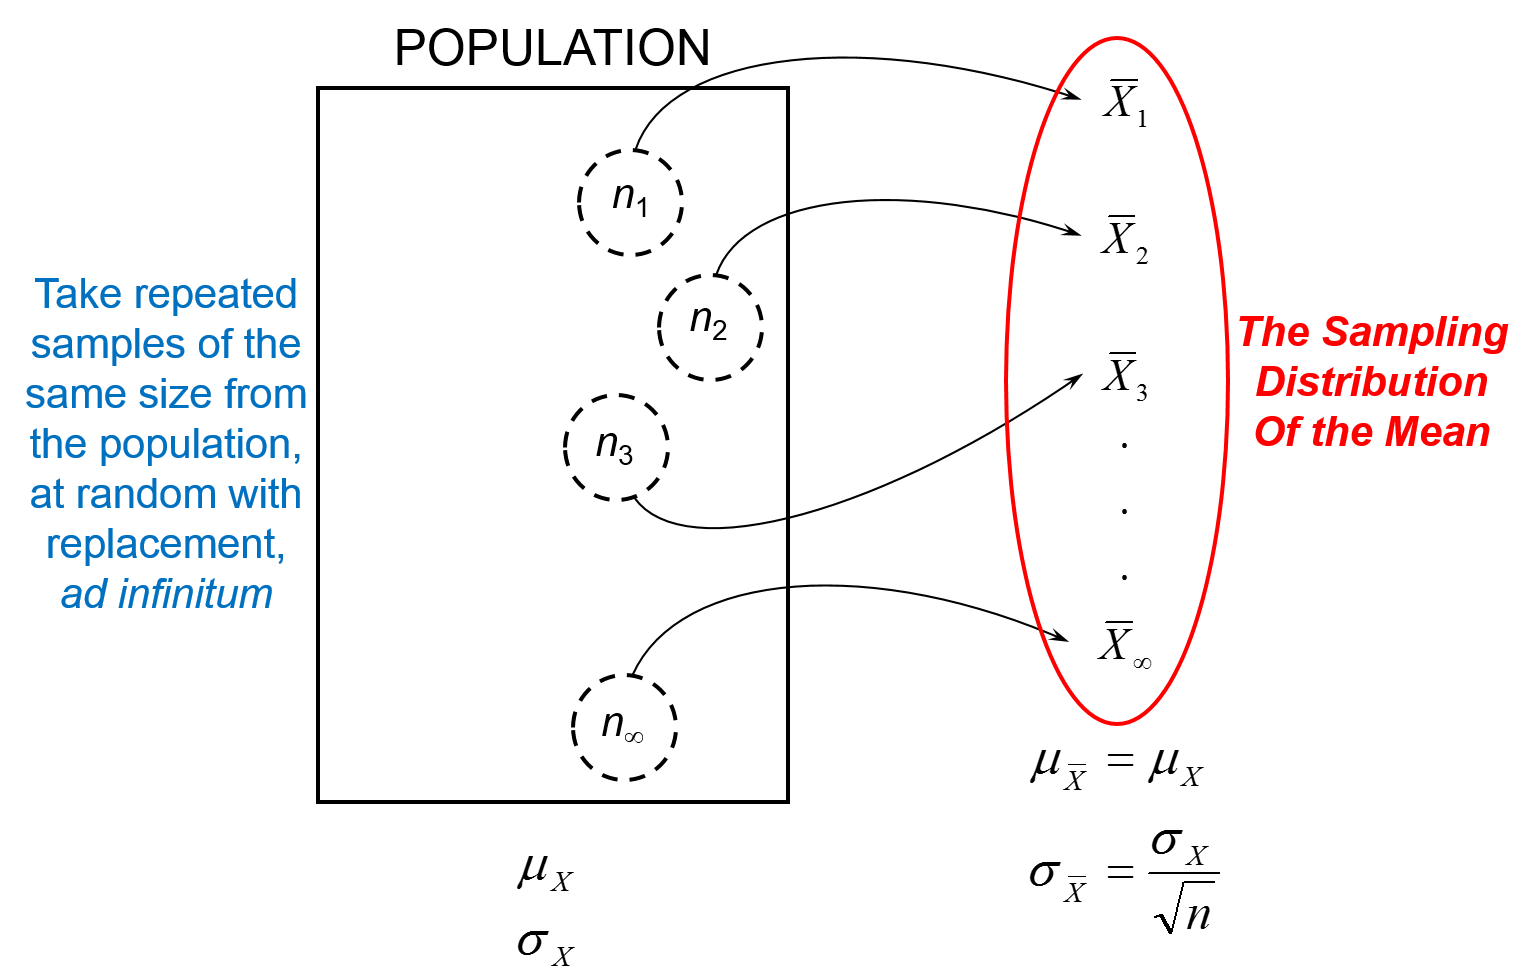
\includegraphics[width=3.5in]{sample_dist_general.png}
\caption{}
\end{figure}

\section{Sampling Distribution Example
2}\label{sampling-distribution-example-2}

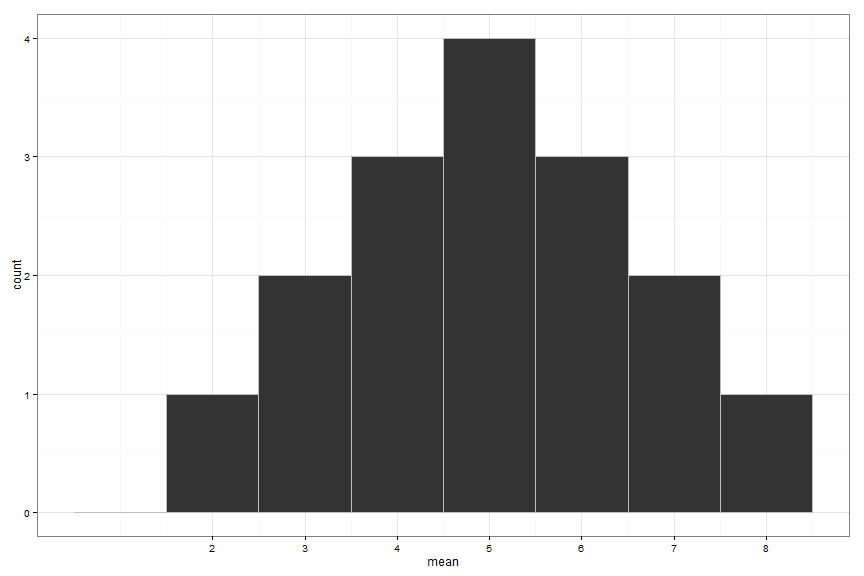
\includegraphics[width=3.5in]{figure/sampdist2-1.png}
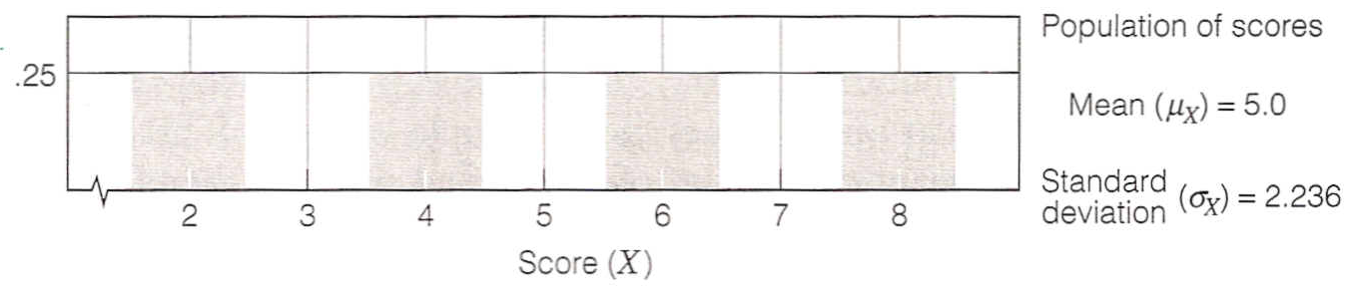
\includegraphics[width=3.5in]{sample_dist_population.png}

\section{Sampling Distribution Example
3}\label{sampling-distribution-example-3}

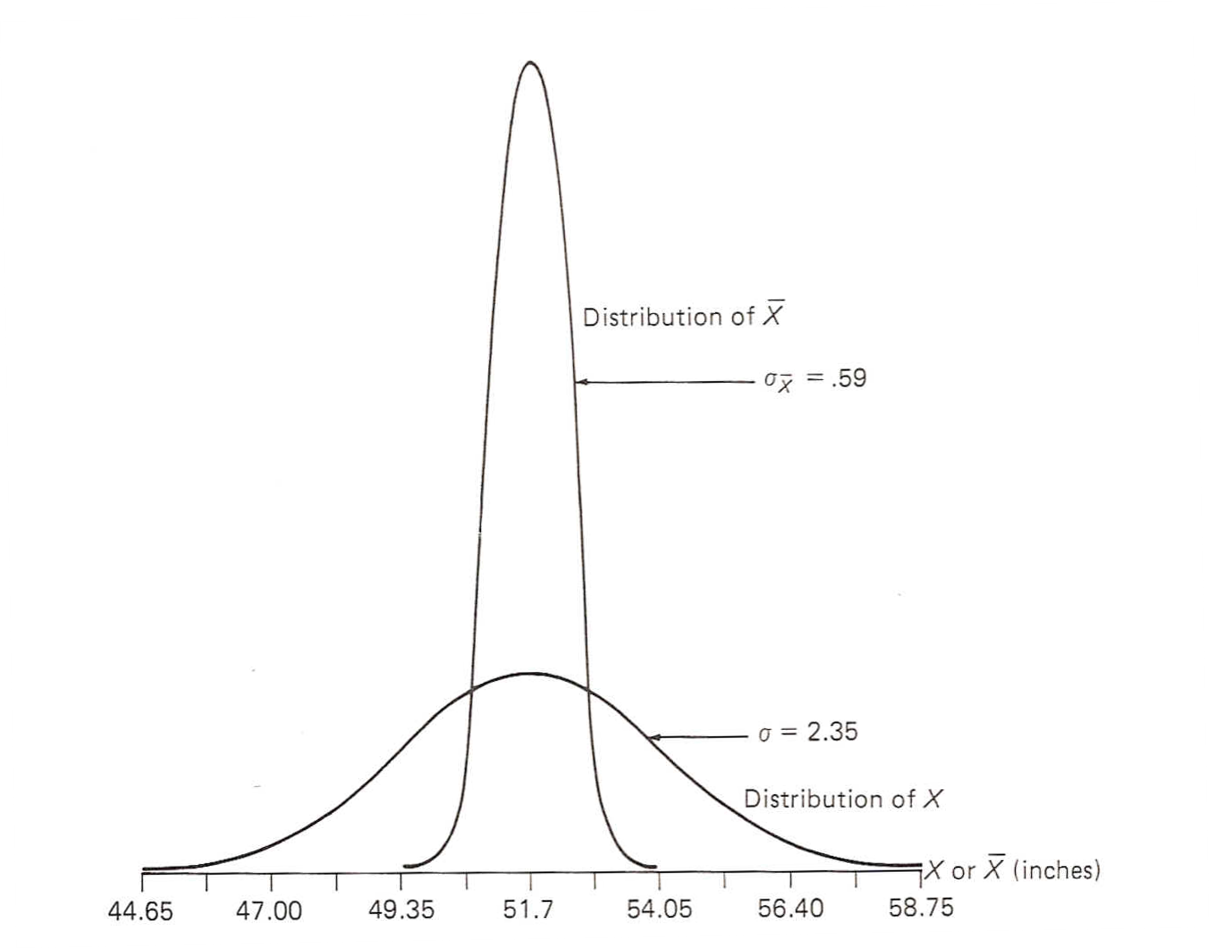
\includegraphics[width=3.5in]{sample_dist_example.png}
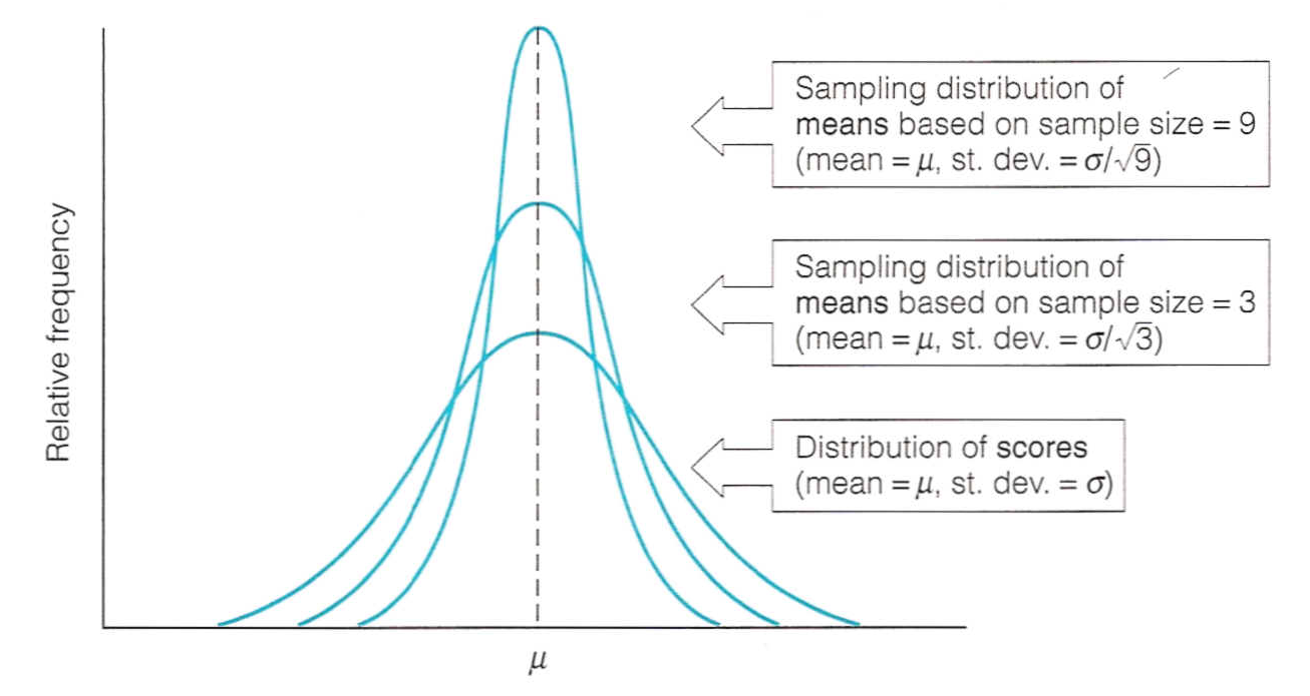
\includegraphics[width=3.5in]{sample_dist_example2.png}

\section{Central Limit Theorem}\label{central-limit-theorem}

\begin{itemize}
\itemsep1pt\parskip0pt\parsep0pt
\item
  The random sampling distribution of the mean \textbf{tends} toward a
  normal distribution \textbf{irrespective of the shape} of the
  population of observations sampled.
\item
  The approximation to the normal distribution improves as sample size
  increases. 
\end{itemize}
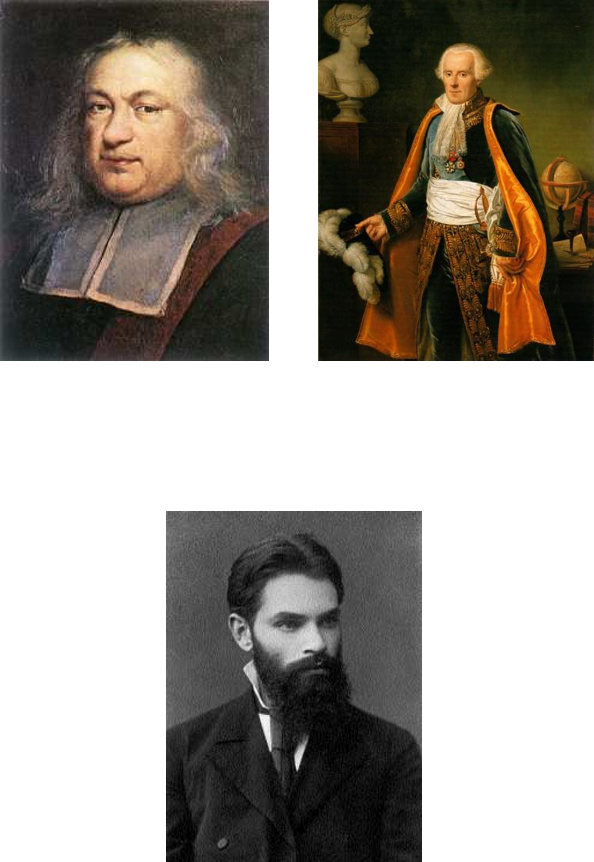
\includegraphics[width=2.5in]{CLT_founders.png}

\section{Central Limit Theorem
Example}\label{central-limit-theorem-example}

\begin{figure}[H]
\centering
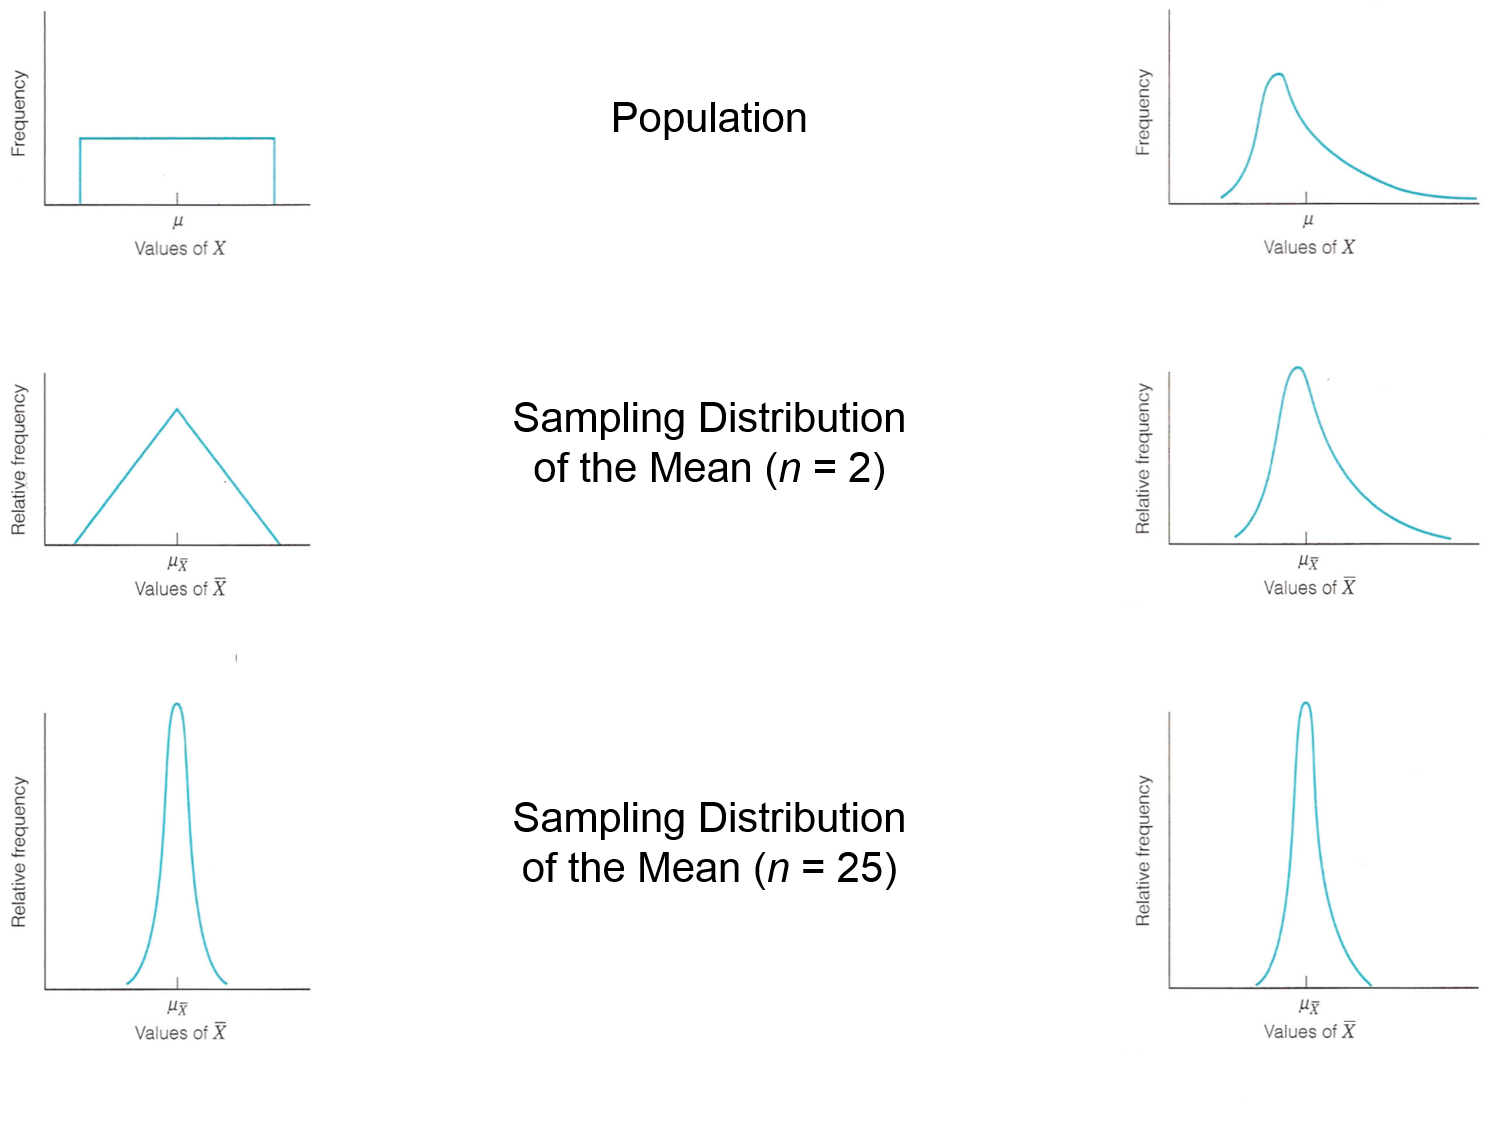
\includegraphics[width=3.5in]{CLT_example.png}
\caption{}
\end{figure}

\section{Central Limit Theorem
Summary}\label{central-limit-theorem-summary}

\begin{itemize}
\itemsep1pt\parskip0pt\parsep0pt
\item
  If raw scores are normally distributed:

  \begin{itemize}
  \itemsep1pt\parskip0pt\parsep0pt
  \item
    Then the sampling distribution of the mean is normally distributed
    regardless of the sample size.
  \end{itemize}
\item
  If raw scores are not normally distributed:

  \begin{itemize}
  \itemsep1pt\parskip0pt\parsep0pt
  \item
    Then the sample distribution of the mean is approximately normally
    distributed.
  \item
    The approximation is usually good enough as long as \(n \geq 25\)
  \item
    The larger the sample, the better the approximation.
  \end{itemize}
\end{itemize}

\section{Examples}\label{examples}

\begin{itemize}
\itemsep1pt\parskip0pt\parsep0pt
\item
  Given a normally distributed population with \(\mu_{X} = 70\) and
  \(\sigma_{X} = 20\); that is \(X \sim N(70, 20)\)
\item
  Assume that we take a random sample of size \(n = 25\)
\end{itemize}

\section{Example 1}\label{example-1}

\begin{itemize}
\itemsep1pt\parskip0pt\parsep0pt
\item
  What is the probability of obtaining a random sample with a mean of 80
  or higher? \[ Pr (\bar{X} \geq 80 | X \sim N(70, 20)) \]
  \[ Pr (\bar{X} \geq 80 | \bar{X} \sim N(70, 4)) \]
\end{itemize}

\section{Example 2}\label{example-2}

\begin{itemize}
\itemsep1pt\parskip0pt\parsep0pt
\item
  What is the probability of obtaining a random sample with a mean that
  differs from the population mean by more than 10 points?
  \[ Pr (\bar{X} \geq 80 or \bar{X} \leq 60 | X \sim N(70, 20)) \]
  \[ Pr (\bar{X} \geq 80 or \bar{X} \leq 60 | \bar{X} \sim N(70, 4)) \]
  \[ Pr (|\bar{X} - \mu_{X}| \geq 10 | \bar{X} \sim N(70, 4)) \]
\end{itemize}

\section{Example 3}\label{example-3}

\begin{itemize}
\itemsep1pt\parskip0pt\parsep0pt
\item
  What sample mean has a value such that the probability of obtaining
  one at least that high in random sampling is .05?
\item
  Find \(\bar{X}_{o}\) such that:
  \[ Pr (\bar{X} \geq \bar{X}_{o} | \bar{X} \sim N(70, 4)) = 0.05 \]
\end{itemize}

\section{Example 4}\label{example-4}

\begin{itemize}
\itemsep1pt\parskip0pt\parsep0pt
\item
  Within what limits would the central 95\% of the sample means fall?
\item
  Find \(\bar{X}_{1}\) and \(\bar{X}_{2}\) such that:
  \[ Pr (\bar{X}_{1} \leq \bar{X} \leq \bar{X}_{2} | \bar{X} \sim N(70, 4)) = 0.95 \]
\end{itemize}

\section{CLT Overview}\label{clt-overview}

\begin{figure}[H]
\centering
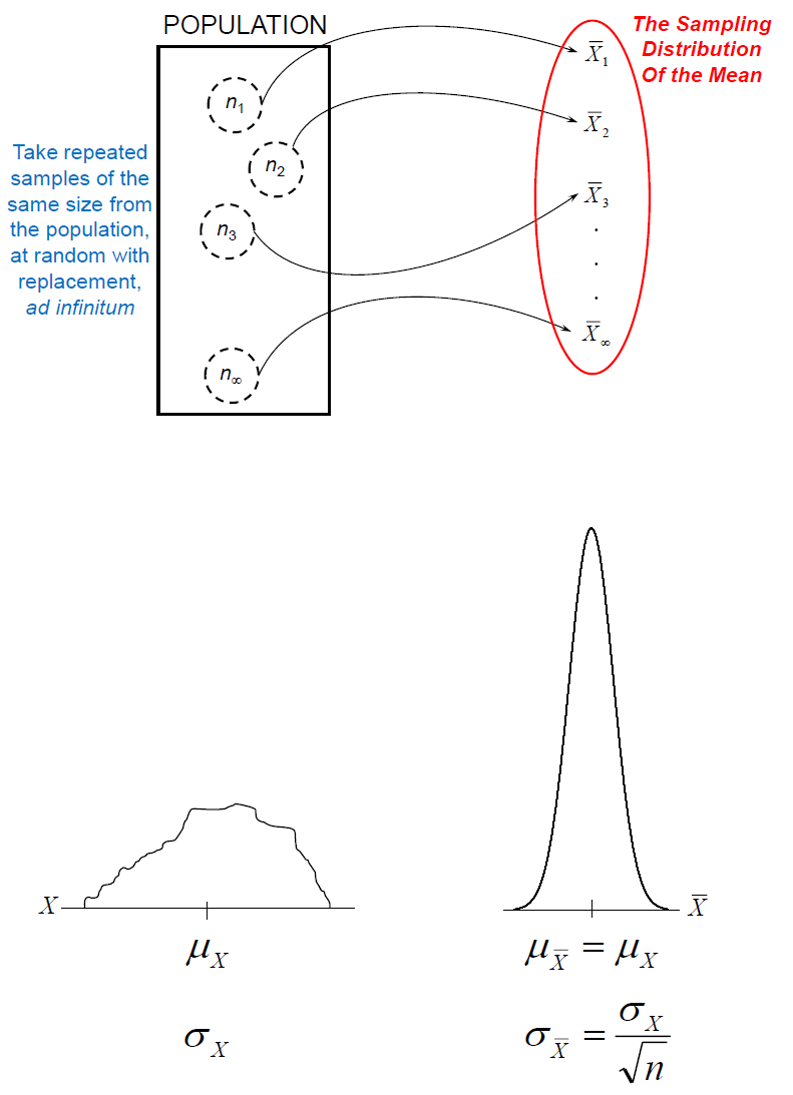
\includegraphics[width=3.5in]{CLT_overview.png}
\caption{}
\end{figure}

\end{document}
